\documentclass{article}
% \documentclass{article}

\usepackage[letterpaper, portrait]{geometry}

\usepackage{amsmath, amsfonts, amsthm, amssymb}
\usepackage{graphicx, float}
\usepackage{mathtools}
\usepackage{siunitx}
\usepackage{esdiff}
\usepackage{titlesec}
\usepackage{multicol}
\usepackage{vwcol}
\usepackage{interval}
\usepackage{afterpage}
\usepackage{tikz}
\usepackage{mdframed}

\intervalconfig {
	soft open fences
}

%opening
\title{Problem Set \#36}
\author{Jayden Li}
% \date{December 15, 2023}

\begin{document}

\newgeometry{top=0.6in, left=0.8in, right=0.8in, bottom=1in}
\maketitle

\fontsize{12pt}{12pt}\selectfont

\section*{Problem 1}
We did this in class on Wednesday, after we finished PS35.

\section*{Problem 2}
\begin{itemize}
\item[(a)]
	\begin{gather*}
		\frac{\sin A}{1+\cos A}+\frac{1+\cos A}{\sin A}
		\stackrel{?}{=}\frac{2}{\sin A}
	\end{gather*}
	\begin{proof}
		$\begin{aligned}[t]
			\text{LHS: }
			\frac{\sin A}{1+\cos A}+\frac{1+\cos A}{\sin A}
			&=\frac{\sin^2A+\left(1+\cos A\right)^2}
				{\left(1+\cos A\right)\sin A} \\
			&=\frac{\sin^2A+1+2\cos A+\cos^2A}
				{\left(1+\cos A\right)\sin A} \\
			&=\frac{1+1+2\cos A}
				{\left(1+\cos A\right)\sin A} \\
			&=\frac{2\left(1+\cos A\right)}
				{\left(1+\cos A\right)\sin A} \\
			&=\frac{2}{\sin A} \\
		\end{aligned} \\$
	\end{proof}

\item[(b)]
	\begin{align*}
		\frac{\sin x}{1+\cos x}+\frac{1+\cos x}{\sin x}&=1+3\sin x \\
		1+3\sin x&=\frac{2}{\sin x} \\
		\sin x+3\sin^2 x&=2 \\
		3\left(\sin^2x+\frac{1}{3}\sin x-\frac{2}{3}\right)&=0 \\
		3\left(\left(\sin x+\frac{1}{6}\right)^2-\frac{1}{36}-
			\frac{2}{3}\right)&=0 \\
		\left(\sin x+\frac{1}{6}\right)^2-\frac{25}{36}&=0 \\
		\sin x+\frac{1}{6}&=\pm\frac{5}{6}
	\end{align*}
	\begin{vwcol}[widths={0.5,0.5},rule=0pt]
		\begin{align*}
			\text{C1: }\sin x+\frac{1}{6}&=\frac{5}{6} \\
			\sin x&=\frac{2}{3}
		\end{align*}
		\[
			\boxed{x=(-1)^{n}\arcsin\frac{2}{3}+\pi n}
		\]
		\vfill\null\pagebreak
		\begin{align*}
			\text{C2: }\sin x+\frac{1}{6}&=-\frac{5}{6} \\
			\sin x&=-1 \\
			x&=(-1)^{n}\arcsin\left(-1\right)+\pi n \\
			\Aboxed{x&=-(-1)^{n}\cdot\frac{\pi}{2}+\pi n}
		\end{align*}
	\end{vwcol}
\end{itemize}


\section*{Problem 3}
\begin{figure}[h]
	\centering
	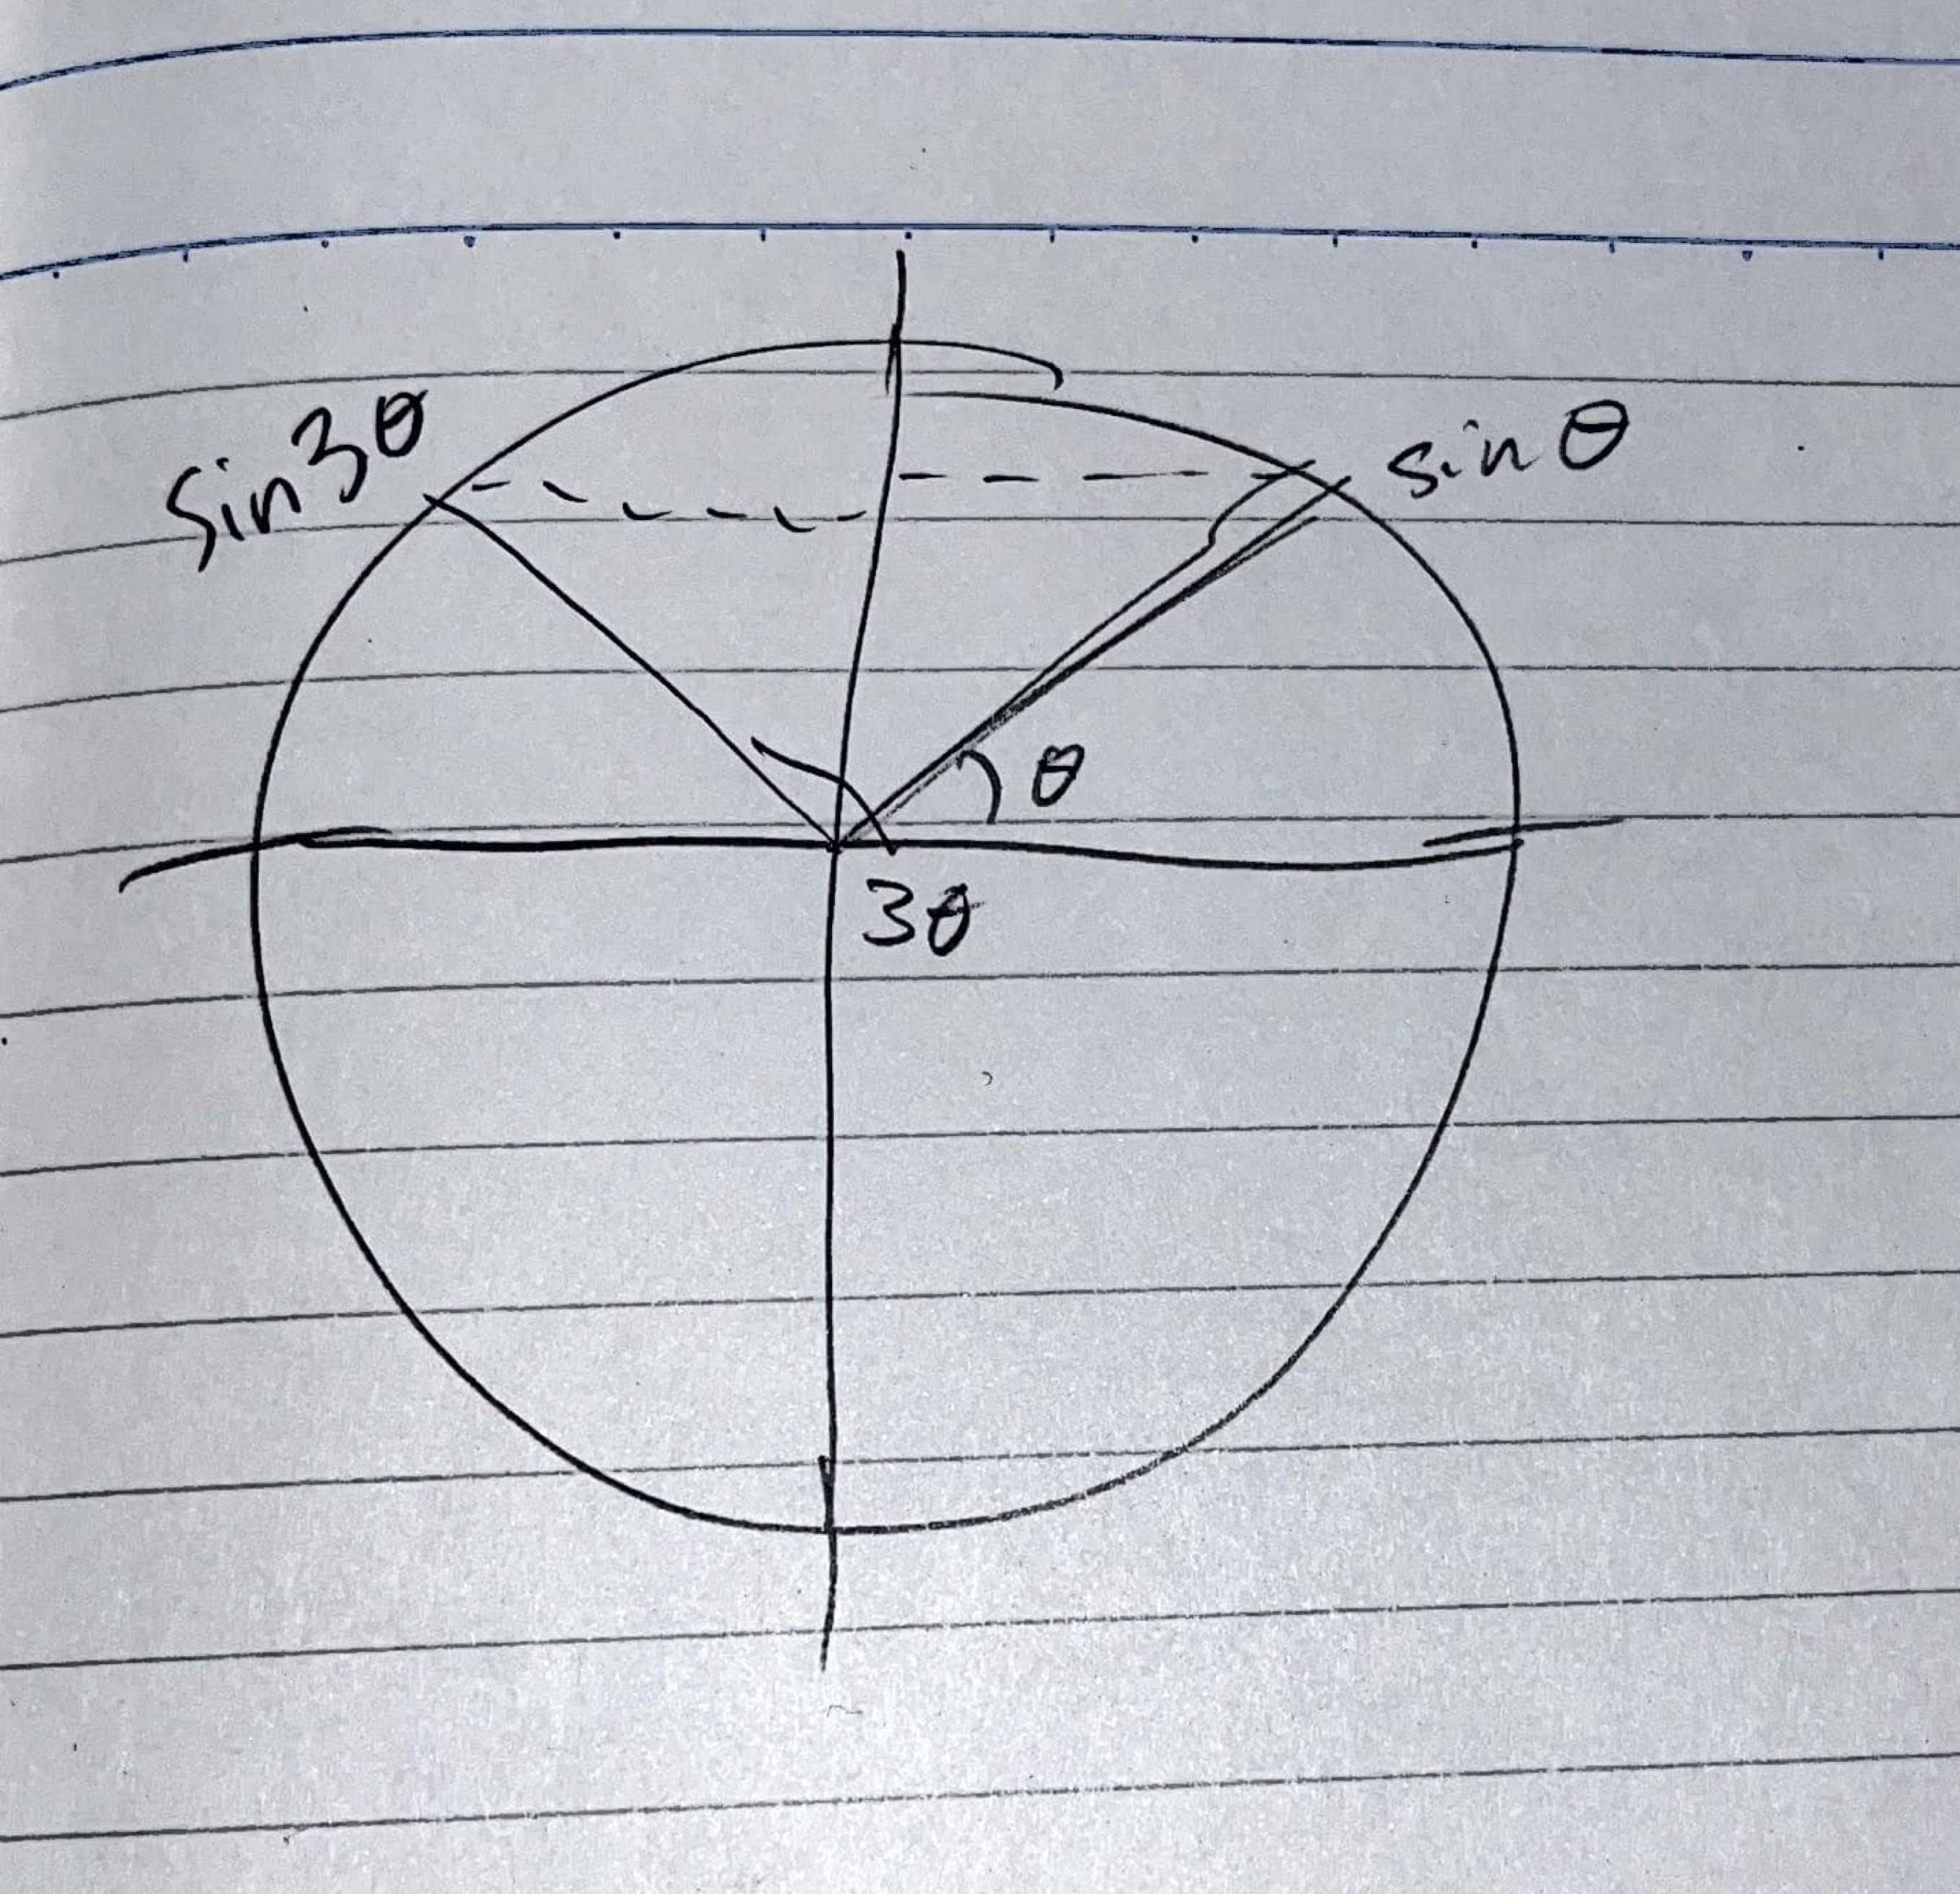
\includegraphics[width=0.5\textwidth]{ps36q3.jpg}
\end{figure}
\begin{align*}
	\sin3\theta&=\sin\left(2\theta+\theta\right) \\
	&=\sin2\theta\cos\theta+\cos2\theta\sin\theta \\
	&=\left(2\sin\theta\cos\theta\right)\cos\theta+
		\left(1-2\sin^2\theta\right)\sin\theta \\
	&=2\sin\theta\cos^2\theta+\sin\theta-2\sin^3\theta \\
	&=\sin\left(\theta\right)
		\left(2\cos^2\theta+1-2\sin^2\theta\right) \\
	&=\sin\left(\theta\right)
		\left(2-2\sin^2\theta+1-2\sin^2\theta\right) \\
	&=\sin\left(\theta\right)\left(3-4\sin^2\theta\right) \\
	\\
	\sin\theta&>\sin3\theta \\
	\sin\theta&>\sin\left(\theta\right)
		\left(3-4\sin^2\theta\right)
\end{align*}
\newpage
\begin{minipage}[t]{.5\textwidth}
	\centering{C1: $\sin\theta>0$}
	\begin{align*}
		1&>3-4\sin^2\theta \\
		4\sin^2\theta&>2 \\
		\sin^2\theta&>\frac{1}{2} \\
		\sin\theta&>\frac{\sqrt{2}}{2}
	\end{align*}
	\begin{gather*}
		\theta\in\interval[scaled,open left,open right]
		{\frac{\pi}{4}+2\pi n}{\frac{3\pi}{4}+2\pi n} \\
	\end{gather*}
	\fbox{$\begin{aligned}
		\theta\in&
		\interval[scaled,open left,open right]{\frac{\pi}{4}
		+2\pi n}{\frac{3\pi}{4}+2\pi n}\,\cup \\
		&\interval[scaled,open left,open right]
		{-\frac{\pi}{4}+2\pi n}{2\pi n}\,\cup \\
		&\interval[scaled,open left,open right]{\pi+2\pi n}
		{\frac{5\pi}{4}+2\pi n}
	\end{aligned}$}
	\vfill\null\pagebreak
\end{minipage}
\begin{minipage}[t]{.5\textwidth}
	\centering{C2: $\sin\theta<0$}
	\begin{align*}
		1&<3-4\sin^2\theta \\
		4\sin^2\theta&<2 \\
		\sin^2\theta&<\frac{1}{2} \\
		\intertext{Only negative case since $\sin\theta$ is
		restricted to be negative in this case. Flip
		inequality sign as a result.}
		\sin\theta&>-\frac{\sqrt{2}}{2}
	\end{align*}
	\begin{gather*}
		\theta\in\interval[scaled,open left,open right]
		{-\frac{\pi}{4}+2\pi n}{\frac{5\pi}{4}+2\pi n}
		\cap\interval[scaled,open left,open right]
		{2\pi n-\pi}{2\pi n} \\
		\theta\in\interval[scaled,open left,open right]
		{-\frac{\pi}{4}+2\pi n}{2\pi n}\cup\interval
		[scaled,open left,open right]{\pi+2\pi n}
		{\frac{5\pi}{4}+2\pi n}
	\end{gather*}
	\vfill\null\pagebreak
\end{minipage}

\section*{Problem 4}
\begin{itemize}

\begin{minipage}[t]{.4\textwidth}
\item[(a)]
	\begin{align*}
		y&=\sin x+\cos x \\
		\diff{y}{x}&=\cos x-\sin x \\
		0&=\cos x-\sin x \\
		\sin x&=\cos x
	\end{align*}
	\[
		\boxed{x=\frac{\pi}{4},\,x=\frac{5\pi}{4}}
	\]
\flushleft
I personally think the Calculus method is more elegant. There
are less steps and the intuition of slope being zero is
simplier. There are also less opportunities for error.
\end{minipage}
\begin{minipage}[t]{.6\textwidth}
\item[(b)]
	\begin{align*}
		y&=\sin x+\cos x \\
		y&=\frac{2}{\sqrt{2}}\left(\frac{\sqrt{2}}{2}\cos x
			+\frac{\sqrt{2}}{2}\sin x\right) \\
		y&=\sqrt{2}\left(\sin\frac{\pi}{4}\cos x
			+\cos\frac{\pi}{4}\sin x\right) \\
		y&=\sqrt{2}\sin\left(\frac{\pi}{4}+x\right)
	\end{align*}
	\flushleft
	The turning points of $\sin\theta$ are when $\sin\theta=1$.
	$\theta=\pi/2$, $\theta=3\pi/2$
	\begin{minipage}[t]{.4\textwidth}
		\begin{align*}
			\frac{\pi}{4}+x&=\frac{\pi}{2} \\
			x&=\frac{2\pi}{4}-\frac{\pi}{4} \\
			x&=\frac{\pi}{4}
		\end{align*}
	\end{minipage}
	\begin{minipage}[t]{.4\textwidth}
		\begin{align*}
			\frac{\pi}{4}+x&=\frac{3\pi}{2} \\
			x&=\frac{6\pi}{4}-\frac{\pi}{4} \\
			x&=\frac{5\pi}{4}
		\end{align*}
	\end{minipage}
	\[
		\boxed{x=\frac{\pi}{4},\,x=\frac{5\pi}{4}}
	\]
\end{minipage}
\end{itemize}

\section*{Problem 5}
\begin{itemize}
\item[(b)]
	\begin{align*}
		2\sin x\cos5x-\cos5x&=0,\,x\in\interval{0}{\pi} \\
		\cos\left(5x\right)\left(2\sin x-1\right)&=0
	\end{align*}
	\begin{minipage}[t]{.5\textwidth}
		\begin{align*}
			\cos\left(5x\right)&=0 \\
			5x&=\pm\arccos\left(0\right)+2\pi n \\
			5x&=\pm\frac{\pi}{2}+2\pi n \\
			x&=\pm\frac{\pi}{10}+\frac{2\pi n}{5} \\
			x&=\frac{\pm\pi+4\pi n}{10}
		\end{align*}
		\begin{gather*}
			x=\frac{\pi}{10},\,\frac{\pi}{2},\,
				\frac{3\pi}{10},\,\frac{9\pi}{10},\,
				\frac{7\pi}{10}
		\end{gather*}
	\end{minipage}
	\begin{minipage}[t]{.5\textwidth}
		\begin{align*}
			2\sin x-1&=0 \\
			\sin x&=\frac{1}{2} \\
			x&=(-1)^n\cdot\arcsin\frac{1}{2}+\pi n \\
			x&=(-1)^n\cdot\frac{\pi}{6}+\pi n
		\end{align*}
		\begin{gather*}
			n=0,\,n=1 \\
			x=\frac{\pi}{6},\,\frac{5\pi}{6}
		\end{gather*}
	\end{minipage}
	\[
	\boxed{x=\frac{\pi}{10},\,\frac{\pi}{2},\,
	\frac{3\pi}{10},\,\frac{9\pi}{10},\,
	\frac{7\pi}{10},\,\frac{\pi}{6},\,\frac{5\pi}{6}}
	\]
\end{itemize}

\section*{Problem 6}
\begin{itemize}
\item[(b)]
	\begin{align*}
		\sin4x-\cos2x&=0 \\
		2\sin2x\cos2x-\cos2x&=0 \\
		\cos\left(2x\right)\left(2\sin2x-1\right)&=0
	\end{align*}
	\begin{minipage}[t]{.5\textwidth}
		\begin{align*}
			\cos2x&=0 \\
			2x&=\pm\arccos\left(0\right)+2\pi n \\
			x&=\frac{1}{2}\left(\pm\frac{\pi}{2}+2\pi n\right)\\
			x&=\pm\frac{\pi}{4}+\pi n
		\end{align*}
	\end{minipage}
	\begin{minipage}[t]{.5\textwidth}
		\begin{align*}
			2\sin2x-1&=0 \\
			\sin2x&=\frac{1}{2} \\
			2x&=(-1)^n\cdot\arcsin\frac{1}{2}+\pi n \\
			x&=(-1)^n\cdot\frac{\pi}{12}+\frac{\pi n}{2}
		\end{align*}
	\end{minipage}
	\[
		\boxed{x=\pm\frac{\pi}{4}+\pi n,\,
		x=(-1)^n\cdot\frac{\pi}{12}+\frac{\pi n}{2}}
	\]

\item[(c)]
	\begin{align*}
		\cos^23x&=\frac{3}{4} \\
		\cos3x&=\pm\frac{\sqrt{3}}{2} \\
		3x&=\pm\arccos\left(\pm\frac{\sqrt{3}}{2}\right)
			+2\pi n
	\end{align*}
	\begin{minipage}[t]{.5\textwidth}
		\begin{align*}
			3x&=\pm\arccos\left(\frac{\sqrt{3}}{2}\right)
			+2\pi n \\
			3x&=\pm\frac{\pi}{6}+2\pi n \\
			x&=\pm\frac{\pi}{18}+\frac{2\pi n}{3}
		\end{align*}
	\end{minipage}
	\begin{minipage}[t]{.5\textwidth}
		\begin{align*}
			3x&=\pm\arccos\left(-\frac{\sqrt{3}}{2}\right)
			+2\pi n \\
			3x&=\pm\frac{5\pi}{6}+2\pi n \\
			x&=\pm\frac{5\pi}{18}+\frac{2\pi n}{3}
		\end{align*}
	\end{minipage}
	\[
		\boxed{x=\pm\frac{\pi}{18}+\frac{2\pi n}{3},\,
		x=\pm\frac{5\pi}{18}+\frac{2\pi n}{3}}
	\]

\item[(d)]
	\begin{align*}
		\sin17x&=\sin7x \\
		17x&=\left(-1\right)^n\cdot\arcsin\left(\sin7x\right)
			+\pi n \\
		17x&=\left(-1\right)^n\cdot7x+\pi n \\
		17x-\left(-1\right)^n\cdot7x&=\pi n \\
		x\left(17-\left(-1\right)^n\cdot7\right)&=\pi n \\
		\Aboxed{x&=\frac{\pi n}{17-7\left(-1\right)^n}}
	\end{align*}

\item[(e)]
	\begin{align*}
		\cos^2x+\sin^23x&=1 \\
		\cos^2x+\sin^23x-\left(\cos^2x+\sin^2x\right)&=1+1 \\
		\cos^2x+\sin^23x-\left(\cos^2x+\sin^2x\right)
			&=1-\left(\cos^2x+\sin^2x\right) \\
		\sin^23x-\sin^2x&=0 \\
		\left(\sin\left(x\right)\left(3-4\sin^2x\right)
			\right)^2-\sin^2x&=0 \\
		\sin^2\left(x\right)\left(3-4\sin^2x\right)^2-
			\sin^2x&=0 \\
		\sin^2\left(x\right)\left(\left(3-4\sin^2x\right)^2
			-1\right)&=0
	\end{align*}
	\begin{minipage}[t]{.3\textwidth}
		\begin{align*}
			\sin^2\left(x\right)&=0
			\sin x&=0 \\
			x&=\pi n
		\end{align*}
	\end{minipage}
	\begin{minipage}[t]{.7\textwidth}
		\begin{align*}
			\left(3-4\sin^2x\right)^2-1&=0 \\
			3-4\sin^2x&=\pm1 \\
			4\sin^2x&=3\pm1 \\
			\sin x&=\pm\frac{\sqrt{3\pm1}}{2}
		\end{align*}
	\end{minipage}
	\begin{minipage}[t]{.33\textwidth}
		\begin{gather*}
			\sin x=1,\,\sin x=-1 \\
			x=\frac{\pi}{2}+2\pi n,\,\frac{3\pi}{2}+2\pi n \\
			x=\frac{\pi}{2}+\pi n
		\end{gather*}
	\end{minipage}
	\begin{minipage}[t]{.33\textwidth}
		\begin{align*}
			\sin x&=\frac{\sqrt{2}}{2} \\
			x&=\left(-1\right)^n\cdot\frac{\pi}{4}+\pi n
		\end{align*}
	\end{minipage}
	\begin{minipage}[t]{.33\textwidth}
		\begin{align*}
			\sin x&=-\frac{\sqrt{2}}{2} \\
			x&=\left(-1\right)^n\cdot\left(-\frac{\pi}{4}
				\right)+\pi n
		\end{align*}
	\end{minipage}
	\[
		\boxed{x=\pi n,\,
			x=\frac{\pi}{2}+\pi n,\,
			x=\left(-1\right)^n\cdot\frac{\pi}{4}+\pi n,\,
			x=-\left(-1\right)^n\cdot\frac{\pi}{4}+\pi n}
	\]
\end{itemize}

\section*{Problem 7}
\begin{itemize}
\begin{minipage}[t]{.45\textwidth}
\item[(b)]
	\begin{align*}
		\cot x&\leq-\sqrt{3} \\
		\frac{\cos x}{\sin x}+\sqrt{3}&\leq0 \\
		\frac{\cos x+\sqrt{3}\sin x}{\sin x}&\leq0 \\
		\frac{2\left(\frac{1}{2}\cos x+
			\frac{\sqrt{3}}{2}\sin x\right)}{\sin x}&\leq0 \\
		\frac{2\left(\sin\frac{\pi}{6}\cos x+
			\cos\frac{\pi}{6}\sin x\right)}{\sin x}&\leq0 \\
		\frac{\sin\left(\frac{\pi}{6}+x\right)}{\sin x}&\leq0 \\
	\end{align*}
	\begin{minipage}[t]{.5\textwidth}
		\begin{align*}
			\sin\left(\frac{\pi}{6}+x\right)&=0 \\
			\frac{\pi}{6}+x&=\arcsin0 \\
			x&=-\frac{\pi}{6}
		\end{align*}
	\end{minipage}
	\begin{minipage}[t]{.32\textwidth}
		\begin{align*}
			\sin x&=0 \\
			x&=\arcsin0 \\
			x&=0
		\end{align*}
	\end{minipage}

	\flushleft
	The range of $\arcsin x$ is $\interval[scaled]
	{-\frac{\pi}{2}}{\frac{\pi}{2}}$, so the periodicity
	is $\pi$.
	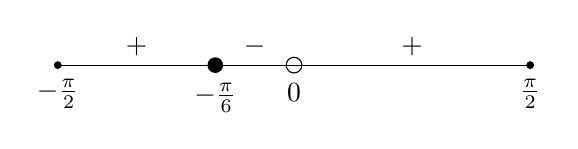
\begin{tikzpicture}	
		\draw
		(0,0) node[circle,fill,inner sep=1pt,label=below:$-\frac{\pi}{2}$](){}
	 -- (2,0) node[circle,fill,inner sep=2pt,label=below:$-\frac{\pi}{6}$](){} node[midway,above]{$+$}
	 -- (3,0) node[circle,draw,inner sep=2pt,label=below:$0$](){} node[midway,above]{$-$}
	 -- (6,0) node[circle,fill,inner sep=1pt,label=below:$\frac{\pi}{2}$](){} node[midway,above]{$+$};
	\end{tikzpicture}
	\[
		\boxed{x\in\interval[scaled,open right]
		{-\frac{\pi}{6}+\pi n}{\pi n}}
	\]
\end{minipage}
\begin{minipage}[t]{.54\textwidth}
	\item[(d)]
		\begin{align*}
			\frac{2\cos x+\sqrt{3}}{\sin\left(2x\right)
				\left(2\sin x-\sqrt{3}\right)}&\leq0
		\end{align*}
		\begin{align*}
			2\cos x+\sqrt{3}&=0 \\
			\cos x&=-\frac{\sqrt{3}}{2}
		\end{align*}
		\[
			x=\frac{5\pi}{6},\,\frac{7\pi}{6}
		\]
		\begin{align*}
			\sin\left(2x\right)
				\left(2\sin x-\sqrt{3}\right)&=0
		\end{align*}
		\begin{minipage}[t]{.49\textwidth}
			$\begin{aligned}[t]
				\sin\left(2x\right)&=0 \\
			\end{aligned}$
			\begin{gather*}
				2x=0,\,\pi,\,2\pi,\,3\pi \\
				x=0,\,\frac{\pi}{2},\,\pi,\,\frac{3\pi}{2} \\
			\end{gather*}
		\end{minipage}
		\begin{minipage}[t]{.49\textwidth}
			$\begin{aligned}[t]
				2\sin x-\sqrt{3}&=0 \\
				\sin x&=\frac{\sqrt{3}}{2} \\
			\end{aligned}$
			\begin{gather*}
				x=\frac{\pi}{3},\,\frac{2\pi}{3} \\
			\end{gather*}
		\end{minipage}
	
		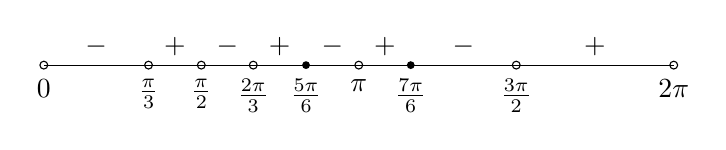
\begin{tikzpicture}	
			\draw
			(0,0) node[circle,draw,inner sep=1pt,label=below:$0$](){}
		 -- (1.33,0) node[circle,draw,inner sep=1pt,label=below:$\frac{\pi}{3}$](){} node[midway,above]{$-$}
		 -- (2,0) node[circle,draw,inner sep=1pt,label=below:$\frac{\pi}{2}$](){} node[midway,above]{$+$}
		 -- (2.66,0) node[circle,draw,inner sep=1pt,label=below:$\frac{2\pi}{3}$](){} node[midway,above]{$-$}
		 -- (3.33,0) node[circle,fill,inner sep=1pt,label=below:$\frac{5\pi}{6}$](){} node[midway,above]{$+$}
		 -- (4,0) node[circle,draw,inner sep=1pt,label=below:$\pi$](){} node[midway,above]{$-$}
		 -- (4.66,0) node[circle,fill,inner sep=1pt,label=below:$\frac{7\pi}{6}$](){} node[midway,above]{$+$}
		 -- (6,0) node[circle,draw,inner sep=1pt,label=below:$\frac{3\pi}{2}$](){} node[midway,above]{$-$}
		 -- (8,0) node[circle,draw,inner sep=1pt,label=below:$2\pi$](){} node[midway,above]{$+$};
		\end{tikzpicture}
		\begin{mdframed}\begin{gather*}
			x\in
			\interval[scaled,open left,open right]
			{2\pi n}{\frac{\pi}{3}+2\pi n}\cup
			\interval[scaled,open left,open right]
			{\frac{\pi}{2}+2\pi n}{\frac{2\pi}{3}+2\pi n}\cup
			\\
			\interval[scaled,open right]
			{\frac{5\pi}{6}+2\pi n}{\pi+2\pi n}\cup
			\interval[scaled,open right]
			{\frac{7\pi}{6}+2\pi n}{\frac{3\pi}{2}+2\pi n}
		\end{gather*}\end{mdframed}
	\end{minipage}

\item[(e)]
	\begin{align*}
		\frac{2\sin x-1}{2\cos x-\sqrt{3}}\geq0
	\end{align*}
	\begin{minipage}[t]{.5\textwidth}
	\begin{minipage}[t]{.4\textwidth}
		\begin{gather*}
			2\sin x-1=0 \\
			\sin x=\frac{1}{2} \\
			x=\frac{\pi}{6},\,\frac{5\pi}{6} \\
		\end{gather*}
	\end{minipage}
	\begin{minipage}[t]{.4\textwidth}
		\begin{gather*}
			2\cos x-\sqrt{3}=0 \\
			\cos x=\frac{\sqrt{3}}{2} \\
			x=\frac{\pi}{6},\,\frac{11\pi}{6} \\
		\end{gather*}
	\end{minipage}

	% \centering
	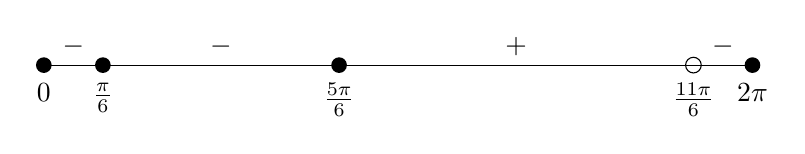
\begin{tikzpicture}	
		\draw
		(0,0) node[circle,fill,inner sep=2pt,label=below:$0$](){}
	-- (0.75,0) node[circle,fill,inner sep=2pt,label=below:$\frac{\pi}{6}$](){} node[midway,above]{$-$}
	-- (3.75,0) node[circle,fill,inner sep=2pt,label=below:$\frac{5\pi}{6}$](){} node[midway,above]{$-$}
	-- (8.25,0) node[circle,draw,inner sep=2pt,label=below:$\frac{11\pi}{6}$](){} node[midway,above]{$+$}
	-- (9,0) node[circle,fill,inner sep=2pt,label=below:$2\pi$](){} node[midway,above]{$-$};
	\end{tikzpicture}
	\end{minipage}
	\begin{minipage}[t]{.29\textwidth}
	\[
		\boxed{x\in\interval[scaled,open right]{\frac{5\pi}
			{6}+2\pi n}{\frac{11\pi}{6}+2\pi n}}
	\]
	\end{minipage}

\end{itemize}

\end{document}
